\nocite{IPbook}

%\cindy{An original comment:
%There's material in this section (e.g. general discussion of combintatorial optimization) that's likely unnecessary for the journal paper. We probably want to start with what is now Section 2, but have some opening introduction giving the big picture.
%Remember when we first mention rounding to be clear this is not numerical rounding. TODO: Add English statement for things currently only given in math. Add definitions of problems so reviewers and readers don't have to look them up.}
\iffalse{
\section{Introduction}\label{chapter:intro}

In combinatorial optimization the aim is to find the optimal solution in a discrete and
usually finite yet large set of solutions. For many specific combinatorial optimization problems such a solution can be found efficiently. For many others, finding optimal or in many cases near optimal solutions is NP-hard. A common approach to deal with such problems is relaxing the discrete solution set into a continuous set, where the optimization problem becomes tractable. Obtaining feasible solutions by means of such a relaxation requires an additional step of rounding the potentially fractional solution of the continuous relaxation into integer solutions.
}\fi

\section{Introduction}
In this paper we focus on finding feasible solutions to binary Integer Linear Programs (IP). Informally, an integer program is the optimization of a linear objective function subject to linear constraints, where the variables must take integer values. Binary variables represent yes/no decisions. Integer Programming (and more generally Mixed Integer Linear Programming (MILP)) can model many practical optimization problems including scheduling, logistics and resource allocation.

It is  NP-hard even to determine if an IP instance has a feasible solution~\cite{GareyJohnson}. Given its practical importance, however, there are many commercial (e.g. CPLEX, GUROBI, XPRESS) and free (e.g. CBC) solvers that for specific IP instances can often find solutions that are optimal within a given tolerance. Still we have formulated moderate-sized IP instances that no commercial solver can currently solve. Thus there is value in heuristics to find feasible solutions for general IP instances (see e.g.~\cite{HanafiT2017}).
%For a generic IP instance $I$ it is NP-hard to even decide if the set of feasible solutions $S(I)$ is empty or not.
%There are a number of heuristics for this purpose, such as the
These heuristics, such as the popular Feasibility pump algorithm \cite{fp1,fp2}, are often effective and fast in practice. However, the heuristics can sometimes fail to find a feasible solution. Moreover, these heuristics do not provide any bounds on the quality of the solution they find. 

\iffalse
However, there is substantial research into finding a feasible, provably-good approximate, and even (computationally) provably optimal solutions to specific IP instances. 
There is substantial research into finding a feasible, provably-good approximate solution for TODO, and even (computationally) provably optimal solutions to specific IP instances. \cindy{TODO: probably need to informally distinguish between a IP for a general problem, and a specific instance when the parameters are set.}
\fi

A major tool for finding feasible solutions for discrete optimization problems expressed as IPs is the {\em linear-programming (LP) relaxation} for the IP formulation. This is a new problem created by relaxing the integrality constraints for an IP instance, allowing the variables to take continuous (rational) values. Linear programs can be solved in polynomial time. The objective value of the linear programming relaxation provides a bound (lower bound for a minimization problem and upper bound for a maximization problem) on the optimal solution to the IP instance. The solutions can also provide some useful global structure, even though the fractional values might not be directly meaningful. 

{\em LP-based approximation algorithms} use LP relaxations to find provably good approximate feasible solutions to IP problems in polynomial time. At the highest level, they involve solving the LP relaxation, using special structure from the problem to find a feasible solution, and proving that the objective value of the solution is no more than $C$ times worse than the bound from the LP relaxation. The approximation factor $C$ can be a constant or depend on the input parameters of the IP, e.g. $O(\log(n))$ where $n$ is the number of variables in the formulation of the IP (the dimension of the problem).

There is an inherent limit to how small $C$ can be for a given IP. The integrality gap for an IP instance is the ratio of the best integer solution to the best solution of the LP relaxation. Any LP-based approximation cannot have an approximation factor $C$ smaller than the integrality gap because there is no feasible solution with an objective value better than a factor of $C$ worse than the optimal solution of the LP relaxation. 

If the integrality gap for an IP formulation is large, it is sometimes possible to add families of constraints to the formulation to reduce the integrality gap.  These constraints are redundant for the integer problem, but can make some fractional solutions no longer feasible for the LP. These families of constraints (cuts) can have exponential size (number of constraints) as long as we can provide a polynomial-time separation algorithm. A separation algorithm for a family of constraints takes an optimal solution to an LP instance that explicitly enforces only a (potentially empty) subset of the family. It either confirms that all constraints are satisfied or returns a most violated constraint. Thus one can add this constraint and repeat at most a polynomial number of times until all are satisfied.

Reducing the integrality gap of an IP formulation has two advantages.  It can lead to better LP-based approximation algorithm bounds as described above.  It can also help exact solvers run faster or solve instances it could not before. Exact IP solvers are based on intelligent branch-and-bound strategies.  As mentioned above, commercial and open-source MILP solvers can find exact solutions (or near-optimal solutions with a provable bound) to many specific instances of NP-hard combinatorial optimization problems. These solvers use the LP relaxation to get lower bounds (for minimization problems).  The search requires exponential time in the worst case. But this search is practically feasible when the solver can prune large amounts of the search space.  This happens when the lower bound for a region of the search space (subproblem) is worse than the value of a known feasible solution.  This requires a way to find a good heuristic solution and it requires good lower bounds that are as close to the actual optimal value of an IP subproblem as possible.

In this paper, we give a method to find feasible solutions for IPs if the integrality gap is bounded. The method is also a tool for evaluating the integrality gap for a formulation.  Researcher can use it to determine whether they should expend effort to find new classes of cuts.  They can also use it to help guide theory for finding tighter bounds on the integrality gap for classic problems like the traveling salesman problem.

% A common approach to Integer programming is considering their linear relaxation.
% \cindy{TODO: this has to move to a logical place in the more formal treatment below:
%For some problems such as the \textsc{Minimum Cost Spanning Tree Problem} there are linear programming relaxations whose basic feasible solutions coincide with  integral solutions, i.e. spanning trees.}

%A common and successful approach is to round these (potentially) fractional solutions into integer solutions for the optimization problem at hand. The Integrality gap of a linear relaxation of an integer programming problem is the worst case ratio between the objective values of the discrete problem and the continuous problem. Equivalently, the integrality gap of the linear programming relaxation is a limit to the rounding approach: rounding a fractional solution into an integer solution incurs a multiplicative cost proportional to the integrality gap. In this paper we study integrality gaps for different combinatorial optimization problems and introduce new rounding algorithms that imply bounds on their respective integrality gaps. 

\iffalse{

Let $S$ denote the set of feasible solutions to a combinatorial optimization problem. For instance, for many problems in network optimization, set $S$ is a subset of $ \{0,1\}^n$ where each coordinate of a point in $S$ indicates the absence or presence of the corresponding edge in a solution, and $n$ is the number of edges in the network. Suppose set $S$ can be described as $S=\{x\in \mathbb{Z}^n: Ax\geq b, x\geq 0 \}$ for some $A\in \mathbb{R}^{m\times n}$ and $b\in \mathbb{R}^m$. (Pure) Integer Programming (IP) asks for $\min_{x\in S}cx$ for some $c\in \mathbb{R}^n$. Integer programming is NP-hard and in fact, it is even NP-complete to decide whether set $S$ is empty or not \cite{GareyJohnson}. The convex hull of $S$ denoted by $\conv(S)$ is the minimal convex set containing $S$ and can be formulated as follows.
\begin{equation*}
\conv(S) =\{\sum_{i=1}^{k} \lambda_i x^i: x^i \in S \text{ for } i =1,\ldots,k,\; \lambda_i \geq 0 \text{ for } i = 1,\ldots,k \text{, and } \sum_{i=1}^{k}\lambda_i = 1\}.
\end{equation*}
\cindy{Since most canonical formulations for IP/LP express variables bounds separately, we should mention here that they are rolled into matrix $A$.}

A fundamental fact in polyhedral theory is that $\min_{c\in S} S = \min_{c\in S} \conv(S)$. Notice that $\conv(S)$ is a polyhedron and optimizing a linear function subject to the points lying in a polyhedron can be done in polynomial time in the number of variables and constraints in the description of $\conv(S)$. Such a description, however, might have exponential size in the description of set $S$.

A natural way to bound the solution to the integer program $\min_{x\in S} cx$ is to relax the integrality constraints. Let $L= \{x\in \mathbb{R}^n: Ax\geq b, x\geq 0\}$. Contrary to integer programming, the optimal solution to $\min_{x\in L}cx$ can be efficiently found. Set $L$ is called the linear programming relaxation of $S$. Since we relaxed the integrality requirement on $x$, we have	
\begin{equation}\label{lp-lower-bound}
\min_{x\in L} cx \leq \min_{x\in S}cx.
\end{equation}
For most relevant applications and for the entirety of this dissertation we assume $c$ is a non-negative vector and  $c\neq 0$, i.e. $c$ has a positive value in at least one coordinate. Following this assumption we can rewrite (\ref{lp-lower-bound}) as 
\begin{equation}
\frac{\min_{x\in S}cx}{\min_{x\in L} cx}\geq 1.
\end{equation}
Since we are concerned with the worst-case analysis, we consider 

\vspace*{5pt}
\noindent\fbox{%
	\parbox{\textwidth}{%
		\vspace*{3pt}
		\begin{equation}\label{eq:IG}
		g=\max_{c\in \mathbb{R}^n_{\geq 0}}\frac{\min_{x\in S}cx}{\min_{x\in L} cx}.
		\end{equation}
	}%
}
\vspace*{3pt}

If $g=1$, we say that the linear programming formulation is a perfect formulation. Otherwise we have $g>1$. In this case, we cannot hope to achieve an integer solution with cost lower than $(g-\epsilon)\cdot (\min_{x\in L}cx)$, for any constant $\epsilon>0$. Thus, a lower bound on $g$ provide a certificate for impossibility of approximation via the linear relaxation for which the gap is $g$. On the other hand, an upper bound of $\alpha$ for $g$ is often accompanied with an $\alpha$-approximation algorithm. This is not always the case, as we will later discuss in details.

We refer to $g$ as the integrality gap of the linear relaxation. For a polyhedron $P\in \mathbb{R}^n$ let the \textit{dominant of $P$} be $\{x\in \mathbb{R}^n: \exists y \in P: x\geq y\}$ and denote it by $\dom(P)$. Goemans \cite{goemansblocking} gave a characterization of integrality gap based on convex combinations when $\conv(S)=\mathcal{D}(\conv(S))$. Carr and Vempala \cite{Carr2004} generalized this characterization.


\vspace*{5pt}
\noindent\fbox{%
	\parbox{\textwidth}{%
		\begin{thm}[\cite{Carr2004}]\label{CV}
			Let $S=\{x\in \mathbb{Z}^n: Ax\geq 0,x\geq 0\}$, and $L= \{x\in \mathbb{R}^n: Ax\geq 0, x\geq 0\}$ be the linear relaxation of $S$. Then
			\begin{equation*}
			\max_{c\in \mathbb{R}^n_{\geq 0}}\frac{\min_{x\in S}cx}{\min_{x\in L} cx}= \min \{\alpha: \alpha\cdot x \in \mathcal{D}(\conv(S)) \text{ for all $x\in L$}\}.
			\end{equation*}
		\end{thm}
	}%
}
\vspace*{5pt}




A polynomial time algorithm for proving an upper bound on integrality gap is called an LP-based approximation algorithm. For many well studied problems, we still do not know the exact integrality gap and the gap between the best known lower bound and the upper bound on the integrality gap are open. In some cases, there are known upper bounds, yet there is no known approximation algorithm, meaning that the proofs do not yield polynomial time algorithms.
}\fi 
We now describe IPs and our methods more formally. The set of feasible points for a pure IP (henceforth IP) is the set
\begin{equation}
S(A,b)= \{x\in \mathbb{Z}^{n}\;:\; Ax\geq b\}  \label{S},
\end{equation}
where matrix $A$ of rationals has $m$ constraints on $n$ variables and $b \in \mathbb{R}^{m}$.
If we drop the integrality constraints, we have the linear relaxation of set $S(A,b)$,
\begin{equation}
P(A,b) = \{x\in \mathbb{R}^{n}\;:\; Ax\geq b\}. \label{P}
\end{equation}
Let $I=(A,b)$ denote an instance. Then $S(I)$ and $P(I)$ denote $S(A,b)$ and $P(A,b)$, respectively. Given a linear objective function $c$, an IP is $\min \;\{cx:\; x \in S(I)\}$. 

Relaxing the integrality constraints gives the polynomial-time-solvable linear programming relaxation: $\min \;\{cx:\;x\in P(I) \}$.  The optimal value of this linear program (LP), denoted $z_{\lp}(I,c)$, is a lower bound on the optimal value for the IP, denoted $z_{\IP}(I,c)$. 

Many researchers (see \cite{davids,vazirani}) have developed polynomial time LP-based approximation algorithms that find solutions for special classes of IPs whose cost are provably at most $C\cdot z_{LP}(I,c)$ for some (possibly constant) function $C$. If the analysis uses the LP bound to prove the approximation quality, then $C$ is at least the integrality gap.
%However, for many combinatorial optimization problems there is a limit to such techniques based on LP relaxations, represented  by the {integrality gap} of the IP formulation.
%\cindy{Arash: Just read and comment it out if you're OK with this. I'm not sure I got an answer for the following questions, so I'll just make it clear this is the definition we use: Does the integrality gap always require positive objective coefficients?  Or is that an extra restriction in our definition?  Is there a reference that has that restriction?} 
%\arash{I looked for a formal definition of integrality gap in the literature this is the most descriptive I've found from \cite{davids} as follows: \textit{the integrality gap of an integer program is the worst-case ratio over all instances of the problem of value of an optimal solution to the integer programming formulalation to value of an optimal solution to its linear programming relaxation.}. Based on this definition I think we are not adding a restriction but we are looking at specific type of IPs arising form problems whose instances have non-negative cost vectors which is not a huge stretch as most combinatorial optimization problems are of this forms.}
\begin{definition}
The integrality gap $g(I)$ for instance $I$ is: $$g(I)= \max_{c\geq 0}\frac{z_{IP}(I,c)}{z_{LP}(I,c)},$$
where $z_{IP}(I,c)$ is the optimal solution to the integer program and $z_{LP}(I,c)$ is the solution to the linear-programming relaxation.
\end{definition}

In general the integrality gap is defined similarly for any objective function, but we wish to be explicit about the class of problems we assume in this paper. For example consider the minimum cost \textsc{2-edge-connected multi-subgraph problem (2EC)}: Given a graph $G=(V,E)$ and $c\in \mathbb{R}^E_{\geq 0}$, 2EC asks for the minimum cost 2-edge-connected subgraph of $G$, with multiedges allowed. A graph is 2-edge-connected if there are at least two edge-disjoint paths between every pair of vertices.  A linear programming relaxation for this problem, known as the {\em subtour-elimination} relaxation, is
 \begin{equation}\min \{cx: \sum_{e\in \delta(U)}x_e \geq 2 \mbox{ for } \emptyset \subsetneq U \subsetneq V,\; x\in [0,2]^{E}\}, 
 \label{eq:subtour}
 \end{equation}
where $\delta(U)$ for vertex subset $U$ is the set of edges that cross the cut defined by $U$.  That is, each $e \in \delta(U)$ has one endpoint in $U$ and the other endpoint in $V-U$.
 In this case the instance-specific integrality gap is the integrality gap of the subtour-elimination relaxation for the 2EC on a graph with $n$ vertices. Alexander et al. \cite{alexander2006integrality} showed this instance-specific integrality gap
%of the subtour elimination relaxation for the 2EC
is at most $\frac{7}{6}$ for instances with $n= 10$ .

The value of $g(I)$ depends on the constraints in~(\ref{S}).  We cannot hope to find solutions for the IP with objective values better than $g(I)\cdot z_{LP}(I,c)$. More generally we can define the integrality gap for a class of instances $\mathcal{I}$ as follows.% In this case, the integrality gap for problem $\mathcal{I}$ is
\begin{equation}\label{gapproblem}
g(\mathcal{I}) = \max_{c\geq 0 , I\in\mathcal{I}}\frac{z_{IP}(I,c)}{z_{LP}(I,c)}.
\end{equation}
For example, the integrality gap of the subtour elimination relaxation for the 2EC is at most $\frac{3}{2}$ \cite{wolsey} and at least $\frac{6}{5}$ \cite{alexander2006integrality}. Therefore, we cannot hope to obtain an LP-based $(\frac{6}{5}-\epsilon)$-approximation algorithm for this problem using this LP relaxation to bound the quality of a feasible solution.

Our methods apply theory connecting integrality gaps to sets of feasible solutions. Instances $I$ with $g(I)=1$ have $P(I)=\conv(S(I))$, the convex hull of the lattice of feasible points. In this case, $P(I)$ is an \textit{integral} polyhedron. The spanning tree polytope of graph $G$, $\st(G)$, and the perfect-matching polytope of graph $G$, $\permat(G)$, have this property (\cite{Edmonds2003,edmondsPM}). Thus the linear-programming relaxation for minimum-cost spanning tree has basic feasible solutions (vertices) that are integral solutions, i.e. spanning trees. For such problems there is an algorithm to express vector $x\in P(I)$ (a feasible LP solution) as a convex combination of points in $S(I)$ (feasible IP solutions) in polynomial time \cite{cons-cara}.
% The number of feasible solutions ($k$) in the convex combination can vary by instance.
%\cindy{Should this proposition just be a corollary of the Carr-Vempala theorem?  Are we going to describe how to do it?  If so, there should be a forward pointer to that discussion.}

%\arash{not exactly: Carr-Vempala don't give a construction. The proposition below is a result of constructive version of Carathedory's theorem which I think is implied by the Ellipsoid algorithm, but there are even faster versions of it. In some way the difference between prop 1 and theorem 2 is our initial motivation for thinking of polynomial construction.}
\begin{proposition}\label{cara}
	If $g(I)=1$, then for $x\in P(I)$ there exists a positive integer $k$ and $\theta \in [0,1]^k$, where $\sum_{i=1}^{k}\theta_i =1$ and $\tilde{x}^i\in S(I)$ for $i\in [k]$ such that $\sum_{i=1}^{k}\theta_i \tilde{x}^i\leq x$. Moreover, we can find such a convex combination in polynomial time.
\end{proposition}

An equivalent way of describing Proposition \ref{cara} is the following Theorem of Carr and Vempala \cite{Carr2004}. The {\em dominant} of $P(I)$, which we denote by $\dom(P(I))$, is the set of points $x'$ such that there exists a point $x\in P$ with $x'\geq x$ in every component. A polyhedron is of \textit{blocking type} if it is equal to its dominant.

\begin{thm}[Carr, Vempala \cite{Carr2004}] \label{CV2}
	We have $g(I) \leq C$ if and only if for  $x\in P(I)$ there exists $\theta \in [0,1]^k$ where $\sum_{i=1}^{k}\theta_i =1$ and $\tilde{x}^i\in \dom(S(I))$ for $i\in [k]$ such that $\sum_{i=1}^{k}\theta_i \tilde{x}^i\leq Cx$.
\end{thm}
Goemans \cite{goemansblocking} first introduced Theorem \ref{CV2} for blocking-type polyhedra. While there is an exact algorithm for problems with gap $1$, as stated in Proposition \ref{cara}, Theorem~\ref{CV2} is existential, with no construction.
%In contrast to Proposition \ref{cara} which implies exact algorithms for problems with a gap of 1, Theorem \ref{CV} does not imply an approximation algorithm, since it does not suggest how to find such a convex combination in polynomial time.
%This points to an interesting open question. 
% We show later, for $I$ with $g(I)<\infty$, the notation of dominant is in fact useful.
\iffalse

\begin{question*}\label{question1}
	Assume reasonable complexity assumptions (such as UGC or $\textrm{P}\neq \textrm{NP}$). Given instance $I$ with $1<g(I)<\infty$ and $(x,y)\in P(I)$, can we find $\theta \in [0,1]^k$, where $\sum_{i=1}^{k}\theta_i =1$ and $(\tilde{x}^i,\tilde{y}^i)\in \dom(\conv(S(I)))$ for $i=1,\ldots,k$ such that $\sum_{i=1}^{k}\theta_i \tilde{x}^i\leq g(I)x$ in polynomial time?
\end{question*}

This seems to be a very hard question. A more specific question is of more interest.

\begin{question}\label{question2}
	Assume reasonable complexity assumptions, a specific problem $\mathcal{I}$ with  $1<g({\mathcal{I}})<\infty$, and $(x,y)\in P(I)$ for some $I\in \mathcal{I}$, can we find $\theta \in [0,1]^k$, where $\sum_{i=1}^{k}\theta_i =1$ and $(\tilde{x}^i,\tilde{y}^i)\in S(I)$ for $i=1,\ldots,k$ such that $\sum_{i=1}^{k}\theta_i \tilde{x}^i\leq g(\mathcal{I})x$ in polynomial time?
\end{question}
Although Question \ref{question2} is wide open, for some problems there are polynomial time algorithms closing the gap. For example, for generalized Steiner forest problem \cite{jain} gave an LP-based 2-approximation algorithm. The gap for this problem is also lower bounded by 2. Same holds for the set covering problem \cite{randomizedrounding}. In fact, for set cover the approximation algorithm achieving the same factor as the integrality gap lower bound, is a \textit{randomized rounding} algorithm. Raghavan and Thompson \cite{randomizedrounding} showed that this technique achieves provably good approximation for many combinatorial optimization problems.  

If we relax Question \ref{question1} (resp. Question \ref{question2}), but multiplying $g(I)$ (resp. $g(\mathcal{I})$) by a factor $C$, they are still very interesting, since they will provide upper bounds on the integrality gap of the instance (resp. the problem). The results in this paper serve this purpose.
\fi
To study integrality gaps, we wish to decompose a suitably scaled linear-programming solution into a convex combination of feasible integer solutions {\bf constructively}.  That is, we ask: assuming reasonable complexity assumptions, given a specific problem $\mathcal{I}$ with  $1<g(\mathcal{I})<\infty$, and $x\in P(I)$ for some $I\in \mathcal{I}$, can we find $\theta \in [0,1]^k$, where $\sum_{i=1}^{k}\theta_i =1$ and $\tilde{x}^i\in S(I)$ for $i\in [k]$ such that $\sum_{i=1}^{k}\theta_i \tilde{x}^i\leq Cx$ in polynomial time? We wish to find the smallest factor $C$ possible.

\subsection{Algorithms and Theory Contributions} 
 
We give a general approximation framework for solving binary IPs.
Consider the set of points described by sets $S(I)$ and $P(I)$ as in (\ref{S}) and (\ref{P}), respectively. Assume in addition that $S(I)\in \{0,1\}^n$ and $P(I)\subseteq [0,1]^n$.
%\cindy{Is it $S(I) \subseteq \{0,1\}^n$?}
For a vector $x\in \mathbb{R}_{\geq 0}^n$ such that $x\in P(I)$, let the {\em support} of $x$ be $\spp(x)= \{i \in [n]: x_i \neq 0\}$. For an integer $\beta$ let $\{\beta\}^n$ be the vector $y\in \mathbb{R}^n$ with $y_i=\beta$ for $i\in [n]$.


In Section~\ref{binaryfdt} we introduce the \textit{Fractional Decomposition Tree Algorithm} (FDT) which runs in polynomial time algorithm. Given a point $x\in P(I)$ FDT produces a convex combination of feasible points in $S(I)$ that are dominated coordinatewise by a ``factor" $C$ times $x$.
% in the coordinates corresponding to $x$.
If $C = g(I)$, it would be optimal. However we can only guarantee a factor of $g(I)^{|\spp(x)|}$. FDT iteratively solves linear programs that are about the same size as the description of $P(I)$.

\begin{restatable}{thm}{binaryFDT}
	\label{binaryFDT}
	Assume $1\leq g(I) 	<\infty$. 	
	The Fractional Decomposition Tree (FDT) algorithm, given $x^*\in P(I)$, produces in polynomial time $\lambda\in [0,1]^k$ and $z^1,\ldots,z^k \in S(I)$ such that $k\leq |\spp(x^*)|$, $\sum_{i=1}^{k}\lambda_i z^i\leq \min(Cx^*,\{1\}^{n})$, and $\sum_{i=1}^{k}\lambda_i = 1$. Moreover, $C\leq g(I)^{|\spp(x^*)|}$.
\end{restatable}

In Section~\ref{domTOIP} we describe a subroutine of the FDT, called the DomToIP algorithm, which finds feasible solutions to any IP with finite gap. This can be of independent interest, especially in proving that a model has unbounded gap.
\begin{restatable}{thm}{DomToIP}
	\label{domtoIP}
	Assume $1\leq g(I) < \infty$. The DomToIP algorithm finds $\hat{x}\in S(I)$ in polynomial time.
\end{restatable}

%\cindy{Arash, please check how I defined $L(I)$.  It was not defined before.}
%\cindy{TODO: This implies we know $g(I)$, which is not true in general.  We should add how we bound/estimate it.  I'll return to this after putting that detail back in core if you (Arash) haven't added it by then.}
%\arash{Isn't $P(I)$ the feasible region defined above. I keep $L(I)$ for now but we can replace it later if needed.} \arash{I fixed below so that I don't imply we know $g(I)$, we also might to clearly state that somewhere?}

Here is how the FDT algorithm works at a high level for an instance $I$ with LP feasible region $P(I)$: in iteration $i$ the algorithm maintains a convex combination of  vectors in $\mathcal{D}(P(I))$ that have a 0 or 1 value for coordinates indexed $0,\ldots,i-1$. Let $y$ be a vector in the convex combination from iteration $i-1$. We solve a linear programming problem that gives us $\theta_0,\theta_1\in [0,1]$ and $y^0,y^1\in \mathcal{D}(P(I))$ such that $y\geq \theta_0 y^0 + \theta_1 y^1$, $\theta_0+\theta_1\leq g(I)$, $y^0_i=0$ and $y^1_i=1$. We then replace $y$ in the convex combination with $\frac{\theta_0}{\theta_0+\theta_1}y^0 +\frac{\theta_1}{\theta_0+\theta_1}y^1$.  Repeating this for every vector in the convex combination from the previous iteration yields a new convex combination of points. It is ``more'' integral because now all vectors in the convex combination are integral in their first $i+1$ elements. If in any iteration there are too many points in the convex combination,  we solve a linear programming problem that ``prunes'' the convex combination. At the end we have a convex combination of integer solutions $\mathcal{D}(P(I))$. For each such solution $z$ we invoke the DomToIP algorithm (see Section \ref{domTOIP}) to find $z'\in S(I)$ where $z'\leq z$.


One can extend the FDT algorithm for binary IPs into covering\footnote{A covering IP has nonnegative constraint matrix, objective coefficients and right-hand side ($A,b,c$).} $\{0,1,2\}$ IPs by losing a factor $2^{|\spp(x)|}$ on top of the loss for FDT. To eradicate this extra factor, we must treat the coordinate $i$ with $x_i=1$ differently. We focus on the 2-edge-connected multi-subgraph graph problem (2EC) defined above.  It's subtour-elimination LP relaxation is given in (\ref{eq:subtour}).
%}: Given a graph $G=(V,E)$ and $c\in \mathbb{R}^{E}_{\geq 0}$ find a 2-edge-connected multi-subgraph of $G$ with minimum cost. The natural linear programming relaxation for this problem is 
%\begin{equation}
%\min \{cx \; : \; x(\delta(U))\geq 2 \; \text{ for }\emptyset \subset U \subset V, \; x\in [0,2]^E\}
%\end{equation}
For input graph $G$, let $\subtour(G)$ denote the feasible region of this LP. Let $\2ec(G)$ be the convex hull of incidence vectors\footnote{The incidence vector $x$ of a 2-edge-connected multigraph has an element for each edge $e$, with $x_e \in \{0,1,2\}$ indicating the number of times edge $e$ appears in the solution.} of 2-edge-connected multi-subgraphs of graph $G$. Following the definition in (\ref{gapproblem}) have
\begin{equation}
g(\2ec) = \max_{c\geq 0 , G}\frac{\min_{x\in \2ec(G)} cx}{\min_{x\in \subtour(G)} cx}.
\end{equation}

\begin{restatable}{thm}{FDTEC}
	\label{FDT2EC}
	Let $G=(V,E)$ and $x$ be an extreme point of  $\subtour(G)$. The FDT algorithm for 2EC produces $\lambda\in [0,1]^k$ and 2-edge-connected multi-subgraphs $F_1,\ldots,F_k$ such that $k\leq 2|V|-1$, $\sum_{i=1}^{k}\lambda_i \chi^{F_i}\leq \min(Cx,\{2\}^n)$, and $\sum_{i=1}^{k}\lambda_i = 1$. Moreover, $C\leq g(\2ec)^{|E_x|}$.
\end{restatable}

\subsection{Experiments.} Although the bounds guaranteed in both Theorems \ref{binaryFDT} and \ref{FDT2EC} are large, in Section~\ref{sec:experiment} we show that in practice, the algorithm can work well for network design problems like those described above. We also show how one might use FDT to investigate the integrality gap for such well-studied problems.
%\cindy{TODO: forward pointers to the sections with more details.}




\subsubsection{Minimum vertex cover problem}

In the \textsc{minimum vertex cover problem (VC)} we are given a graph $G=(V,E)$ and $c\in \mathbb{R}^E_{\geq 0}$. A subset of $U$ of $V$ is a \textit{vertex cover} if for all $e\in E$ at least one endpoint of $e$ is in $U$. The goal in VC is to find the minimum-cost vertex cover. The linear programming relaxation for VC is
\begin{equation}
\min \{cx \; : \; x_u + x_v \geq	 1 \text{ for all } e=uv \in E, \; x\in [0,1]^{V}\}.
\end{equation}
The integrality gap of this formulation is exactly 2 \cite{davids}. Austrin, Khot and Safra~\cite{UGhardVC} show that it is UG-hard to approximate VC within any factor strictly better than 2. We compare  FDT and the feasbility pump heuristic \cite{fp1} on the small instances of the PACE\footnote{ Parameterized Algorithms and Computational Experiments: \url{https://pacechallenge.org/2019/}} 2019 challenge test cases \cite{PACE}. FDT was 3-5x slower, but still ran in seconds. It always gave a better vertex cover. For some instances the FDT solution's relative gap with respect to the optimal was half that of feasibility pump.
\subsubsection{Tree augmentation problem}
In the \textsc{Tree Augmentation Problem (TAP)} we are given a  graph $G=(V,E)$, a spanning tree $T$ of $G$ and a cost vector $c\in \mathbb{R}^{E\setminus T}_{\geq 0}$. A subset $F$ of $E\setminus T$ is called a \textit{feasible augmentation} if $(V,T\cup F)$ is a 2-edge-connected graph. In TAP we seek the minimum cost feasible augmentation. The natural linear programming relaxation for TAP is 
\begin{equation}
\min \{cx\; : \; \sum_{\ell \in \cov(e)} x_{\ell} \geq 1 \text{ for } e\in T, \; x\in [0,1]^{E\setminus T}\}.
\end{equation}
where $\cov(e)$ for $e \in T$ is the set of edges $\ell \in E\setminus T$ such that $e$ is in the unique cycle of $T\cup \{\ell\}$. Another way to think of $\cov(e)$ is that if we remove edge $e$ from tree $T$, this partitions the vertices into two connected sets $U$ and $V-U$.  Then $\cov(e) = \delta(U)$ is the set of edges $\ell \neq e$ that cross the cut between $U$ and $V-U$, and whose addition would reconnect the tree. We call the LP above the cut LP. The integrality gap of the cut LP is known to be between $\frac{3}{2}$ \cite{32gaptap} and $2$ \cite{FJ81}. We create random fractional extreme points of the cut LP and apply FDT to find integral solutions. For our instances, the ratio of the value of the feasible solution to the LP lower bound is always below $\frac{3}{2}$. This provides evidence that the integrality gap for such instances may be less than $\frac{3}{2}$.

\subsubsection{2-edge-connected multi-subgraph problem}
Known polyhedral structure makes it easier to study integrality gaps for such problems. We use the idea of fundamental extreme point \cite{carrravi,boydcarr,Carr2004} to create the ``hardest'' LP solutions to decompose.

There are fairly good bounds for the integrality gap for the Traveling Salesman Problem (TSP, see \cite{tspbook}) or 2EC 
%\cindy{We don't define the TSP, though probably don't need to since that really is so classical, and we don't mention it again.  We could consider citing the TSP book.}
Benoit and Boyd~\cite{TSPcompute} used a quadratic program to show the integrality gap of the subtour elimination relaxation for the TSP, $g(\tsp)$, is at most $\frac{20}{17}$ for graphs with at most 10 vertices. Alexander et al. \cite{alexander2006integrality} used the same ideas to provide an upper bound of $\frac{7}{6}$ for $g(\2ec)$ on graphs with at most 10 vertices. 

Consider a graph $G=(V,E)$. A \textit{Carr-Vempala point} $x\in \mathbb{R}^E$ is a fractional point in $\subtour(G)$ where the edges $e$ with $0<x_e<1$ form a single cycle in $G$ and the vertices on the cycle are connected via vertex-disjoint paths of edges $e$ with $x_e =1$ (see Figure \ref{fig:CVpoint})
%\cindy{Every pair of vertices on the cycle is connected this way? It sounds like that, though I don't recall that being necessary. We probably have a figure from an old version we could include if it's not too much trouble.  This will help reviewers and future readers understand much more easily, especially that there could be far more than 12 vertices in the overall solution.}

\arash{I added this figure \ref{fig:CVpoint} but maybe we can put it later in the experiments section to make the introduction shorter?} \cindy{Yes that would be fine, if the reader could also use that figure then.  They could page forward to see the figure when reading the introduction.}

\begin{figure}
\centering
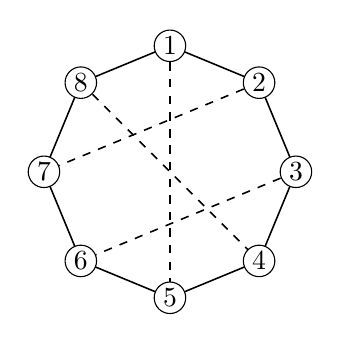
\begin{tikzpicture}[scale=0.4]


\draw [dashed] [black, line width=0.2mm] plot [smooth, tension=0] coordinates {(0,4) (0,-4)};
\draw [dashed] [black, line width=0.2mm] plot [smooth, tension=0] coordinates {(2.83,2.83) (-4,0)};
\draw [dashed] [black, line width=0.2mm] plot [smooth, tension=0] coordinates {(4,0) (-2.83,-2.83)};
\draw [dashed] [black, line width=0.2mm] plot [smooth, tension=0] coordinates {(-2.83,2.83) (2.83,-2.83)};

\draw [-] [black, line width=0.2mm] plot [smooth, tension=0] coordinates {(0,4) (2.83,2.83)};

\draw [-] [black, line width=0.2mm] plot [smooth, tension=0] coordinates {(4,0) (2.83,2.83)};


\draw [-] [black, line width=0.2mm] plot [smooth, tension=0] coordinates {(4,0) (2.83,-2.83)};

\draw [-] [black, line width=0.2mm] plot [smooth, tension=0] coordinates {(0,-4) (2.83,-2.83)};

\draw [-] [black, line width=0.2mm] plot [smooth, tension=0] coordinates {(0,-4) (-2.83,-2.83)};

\draw [-] [black, line width=0.2mm] plot [smooth, tension=0] coordinates {(-4,0) (-2.83,-2.83)};

\draw [-] [black, line width=0.2mm] plot [smooth, tension=0] coordinates {(-4,0) (-2.83,2.83)};

\draw [-] [black, line width=0.2mm] plot [smooth, tension=0] coordinates {(0,4) (-2.83,2.83)};


\draw[black,fill=white] (0,4) ellipse (0.5 cm  and 0.5 cm);
\draw[black,fill=white] (4,0) ellipse (0.5 cm  and 0.5 cm);
\draw[black,fill=white] (0,-4) ellipse (0.5 cm  and 0.5 cm);
\draw[black,fill=white] (-4,0) ellipse (0.5 cm  and 0.5 cm);
\draw[black,fill=white] (2.83,2.83) ellipse (0.5 cm  and 0.5 cm);
\draw[black,fill=white] (-2.83,-2.83) ellipse (0.5 cm  and 0.5 cm);
\draw[black,fill=white] (2.83,-2.83) ellipse (0.5 cm  and 0.5 cm);
\draw[black,fill=white] (-2.83,2.83) ellipse (0.5 cm  and 0.5 cm);

\node (1) at (0,4) {{1}};
\node (2) at (2.83,2.83) {{2}};
\node (3) at (4,0) {{3}};
\node (4) at (2.83,-2.83) {{4}};
\node (5) at (0,-4) {{5}};
\node (6) at (-2.83,-2.83) {{6}};
\node (7) at (-4,0) {{7}};
\node (8) at (-2.83,2.83) {{8}};
\end{tikzpicture}
\caption{A Carr-Vempala point with 8 vertices on its cycle. Solid lines are edges with value strictly between $0$ and $1$. Dashed edges represent paths where each edge on the path has $x_e =1$. There can be an arbitrary number of degree-$2$ vertices on the dashed paths.}
\label{fig:CVpoint}
\end{figure}



Carr and Vempala \cite{Carr2004} showed that $g(\2ec)$ is achieved for instances where the optimal solution to $\min_{x\in \subtour(G)}cx$ is a Carr-Vempala point. We show that the integrality gap is at most $\frac{6}{5}$ for Carr-Vempala points with at most 12 vertices on the cycle formed by the fractional edges.
\cindy{This sounds like a contribution of the paper.} \arash{Yes, particlarly since a similar research question have been studied by \cite{alexander2006integrality} and \cite{TSPcompute}}
Note that the number of vertices in these instances can be arbitrarily high since the paths of edges with $x$-value 1 can be arbitrarily long.

\cindy{We probably need an explicit list of contributions.  It could be another subsection of the introduction.  This will help the reviewer and eventually, if published, the reader.}



